% !TEX root = DesignDoc.tex

\chapter{Mechanical Design}
\label{chap:mechdesign}

This chapter details the mechanical design, as well as the reason behind some of the decisions that were made regarding the mechanical design.\\

Unfortunately for this document's usefulness as a stylistic guide, the mechanical design was mostly just restricted to the chassis available in the lab. However, I will provide some pictures of the SMP, as well as what information I can about the mechanical design.

\section{Surface Mobility Platform}

The Surface Mobility Platform "SMP" is a chassis developed by Gears Educational Systems. The design provides independent suspension for the left and right sides of the robot, allowing it to articulate surprisingly far while maintaining balance and traction.

\begin{figure}[h]
\centering
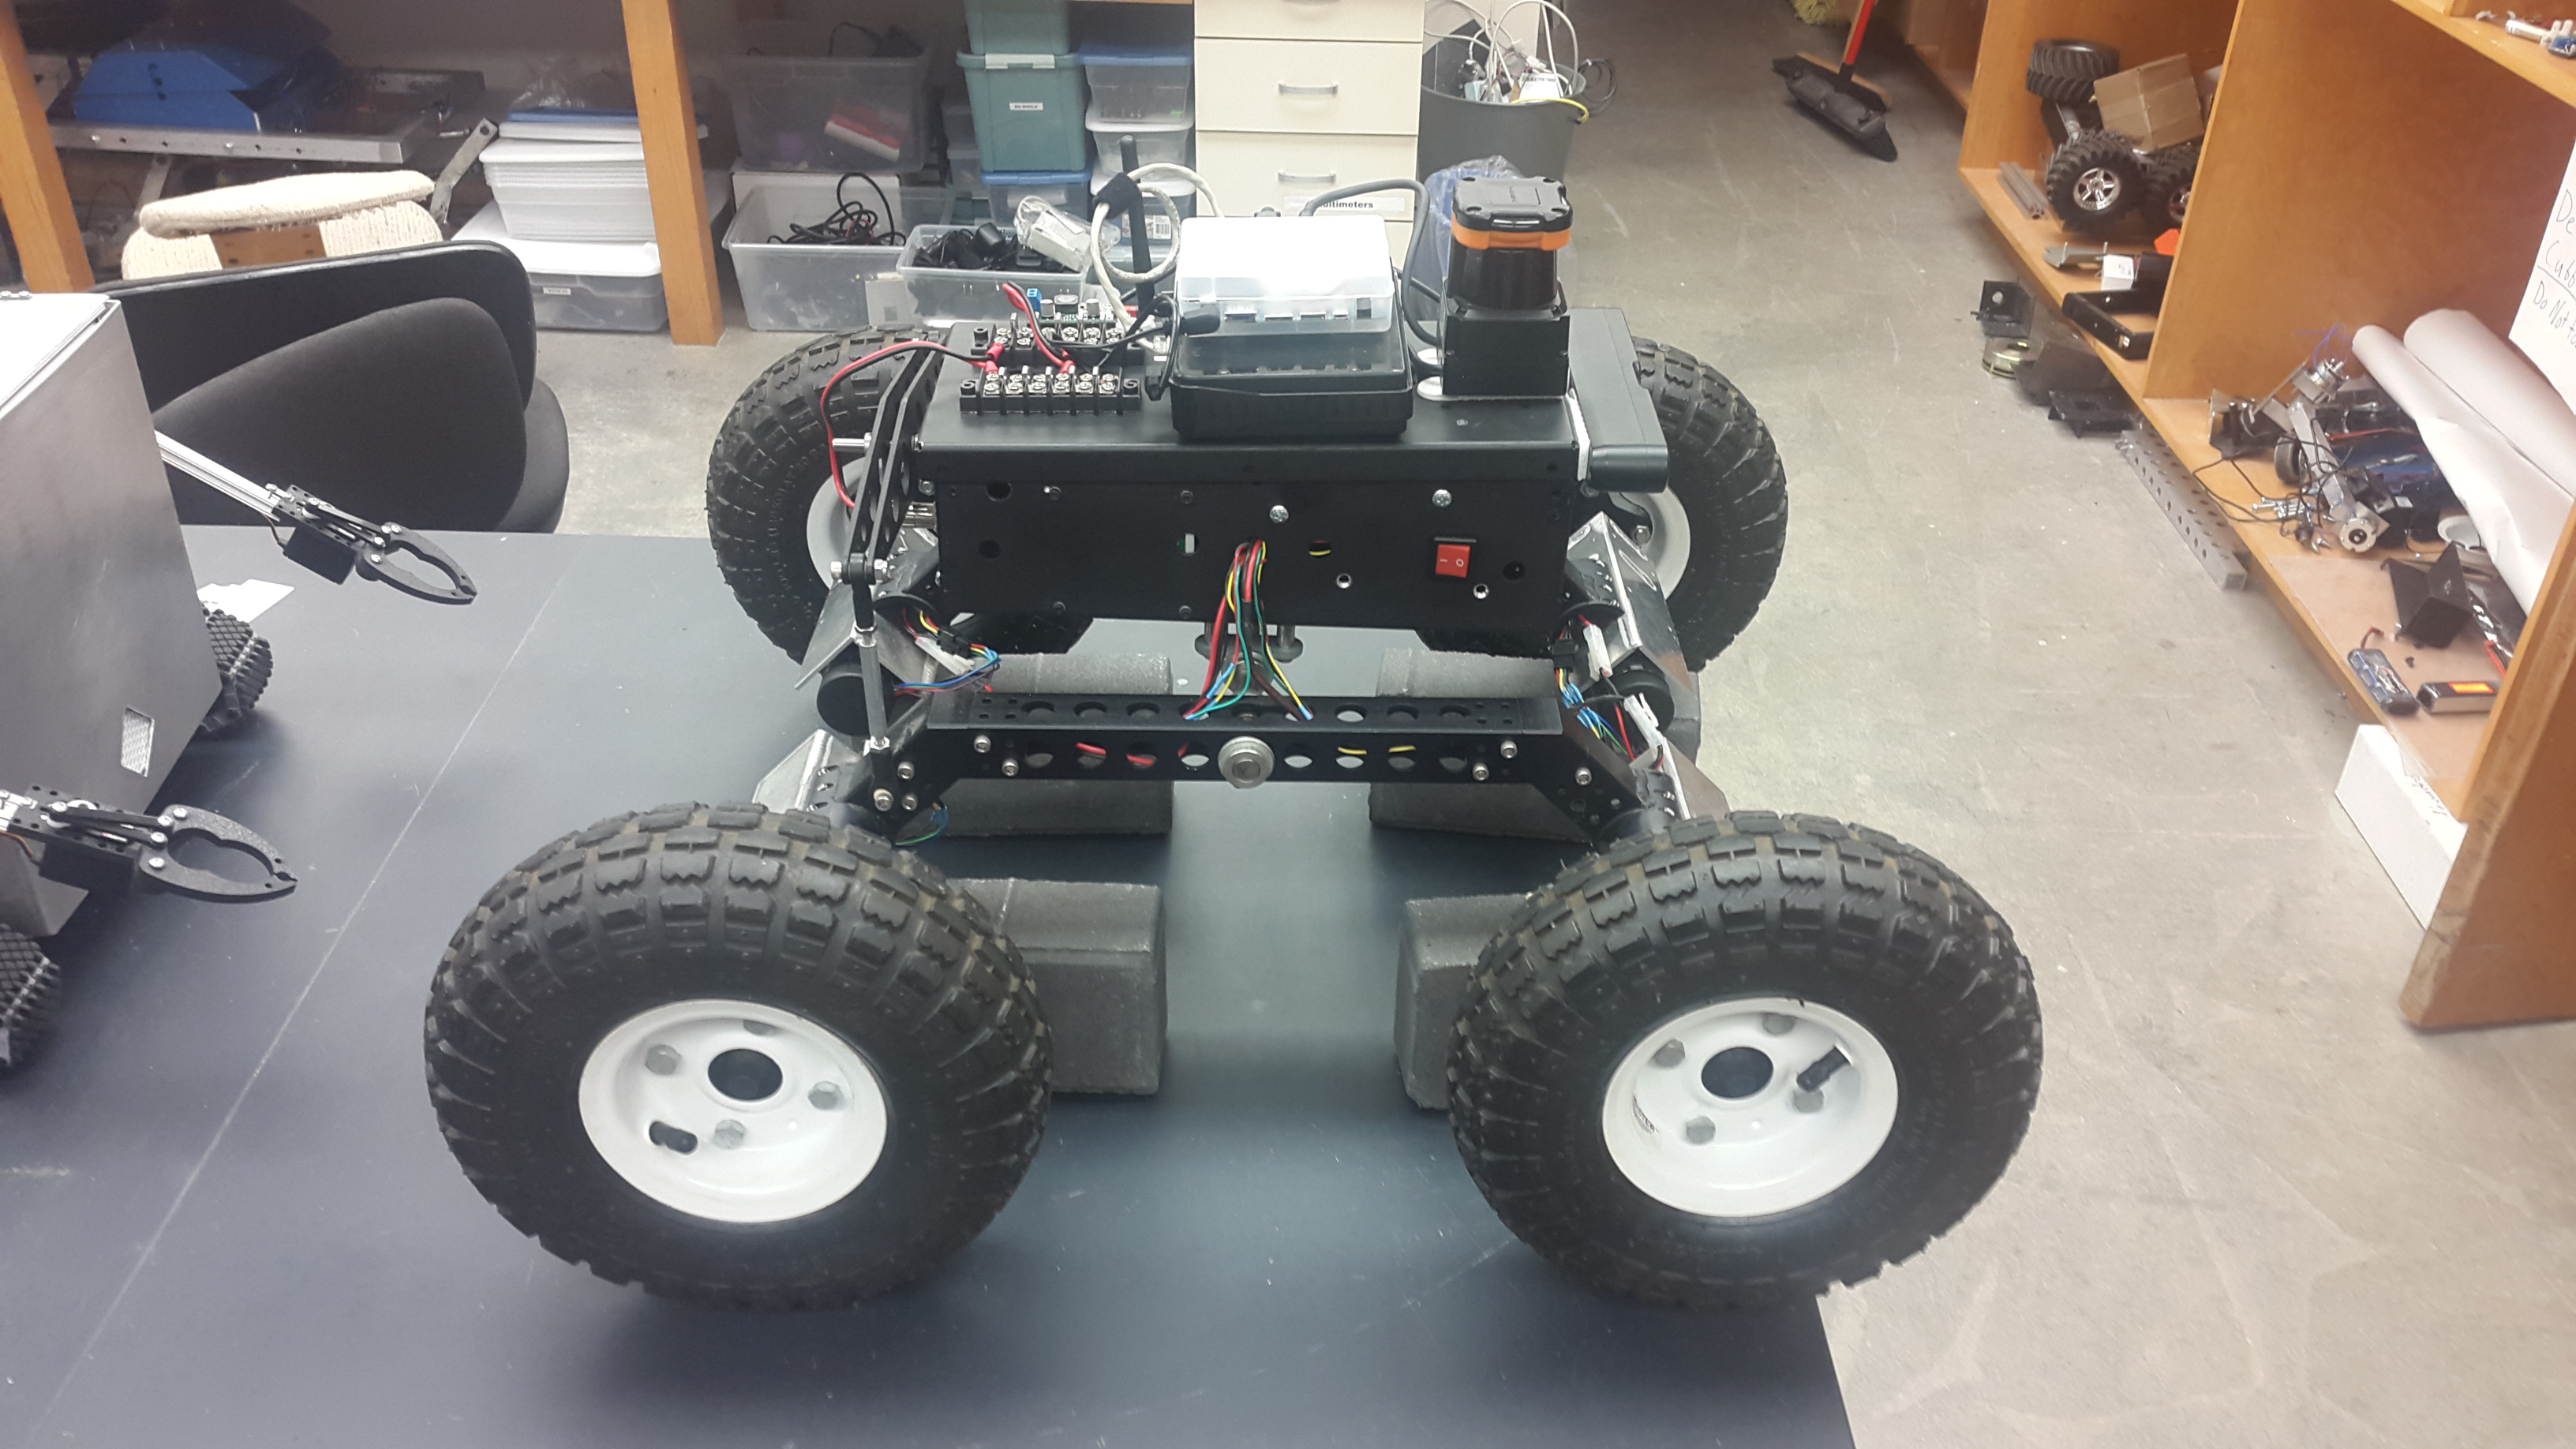
\includegraphics[width=\textwidth]{SMP1.png}
\label{fig:smp1}
\caption{The Suface Mobility Platform "SMP"}
\end{figure}

The silver motor-housings are not part of the original packages. It was determined (at some point in the past) that the stock motors were undesirable for some reason or another. It was a good idea conceptually, but could have used some work in implementation. The screws are difficult to reach, and the housings themselves are not very square. This makes the robot slightly lopsided, which is unfortunate because the rest of the frame is actually really cool.

\begin{figure}[h]
\centering
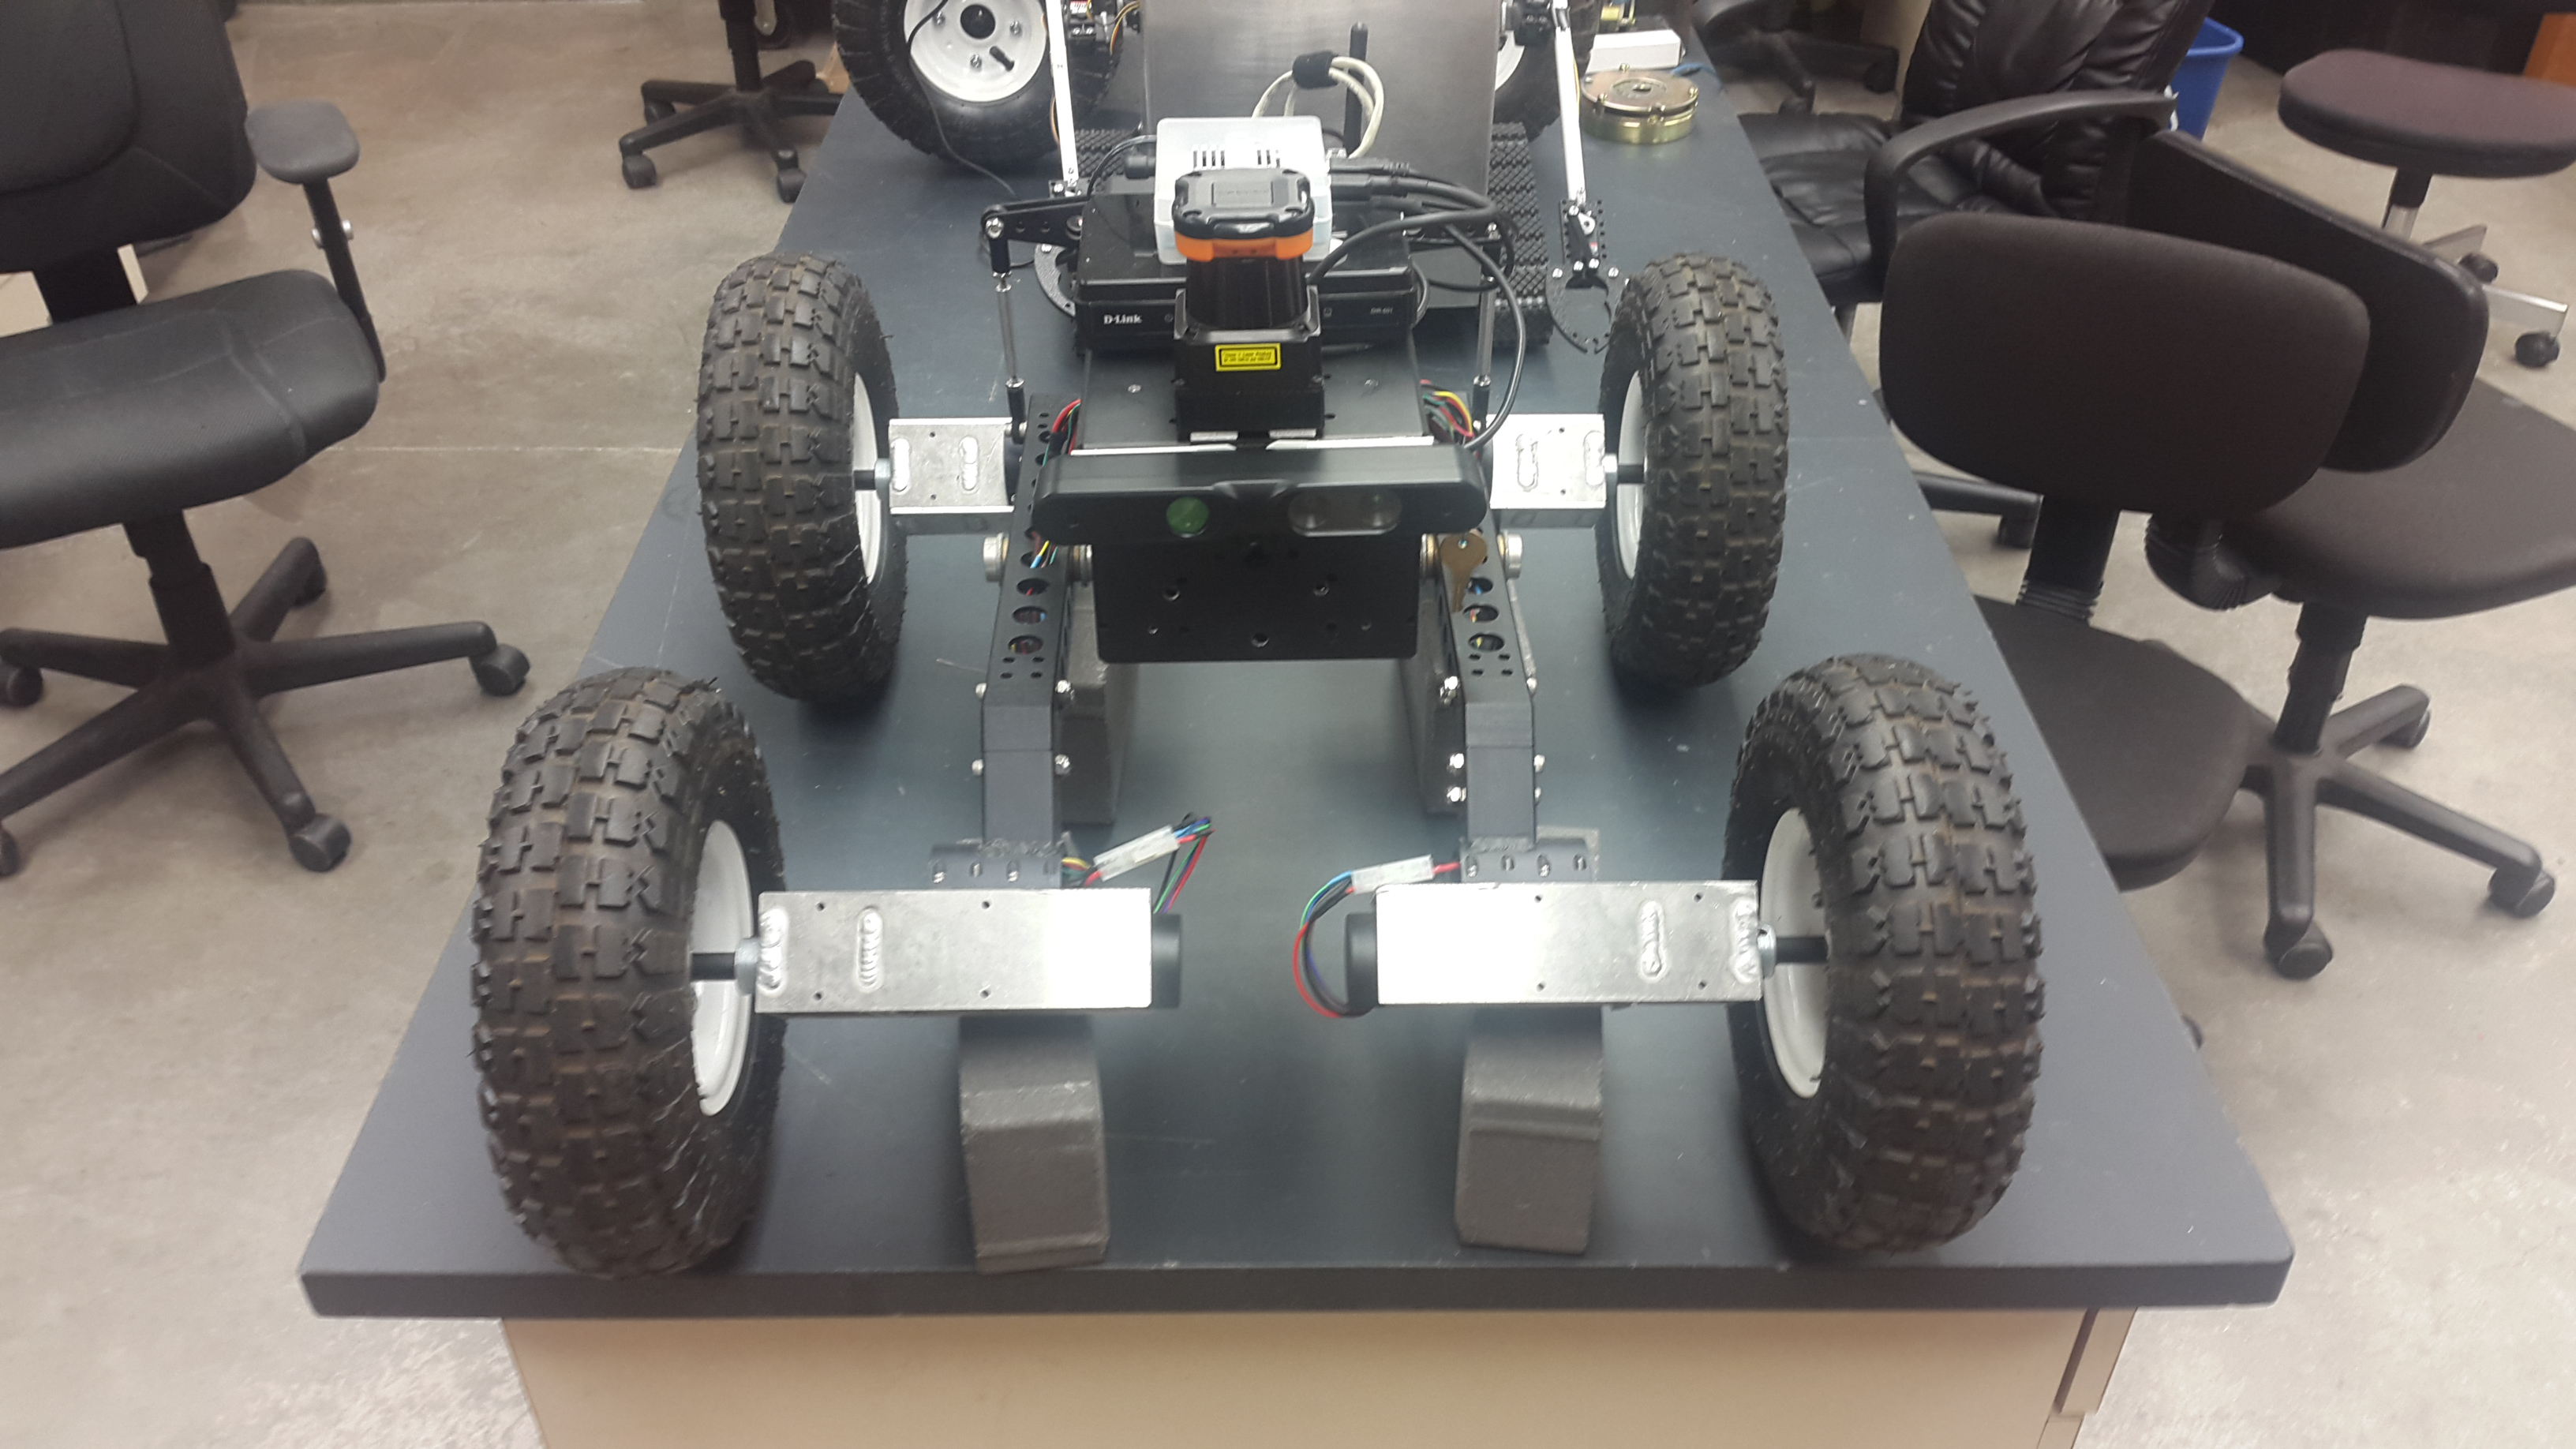
\includegraphics[width=\textwidth]{SMP2.png}
\label{fig:smp2}
\caption{The Suface Mobility Platform "SMP"}
\end{figure}

The SMP uses an aluminum box - now with far too many holes drilled in it - for the main body. The interior of this box is used to house all of the electrically noisy components, creating a sort of Faraday cage to protect the more sensitive electronics, mounted on the top.

To my eternal regret, we decided at the last minute that 3M velcro-tape would be a good mounting solution, as it was easy, didn't require drilling more holes, and made reconfiguration painless. It works ok, but the tape was far more sensitive to vibration and shear stresses than our original tests led us to believe. That being said, it was basically the only way we were able to get everything to fit. Even just putting a few bolts into the box took away too much space inside.

We considered replacing the box currently used for the main body with a larger one, but the articulating bars worked against us. Making the box any wider will cause it to collide with the bars during even fairly low levels of articulation. Making the box longer would both require redesign of the swing arm and pivot joints, as well as looking a bit odd. Making the box taller would raise the center of gravity and put any reasonable mounting points for a LiDAR too far up to be of any real use.

The LiDAR is the piece of main concern with the current mounting system. The wireless router and Odroid are long, wide, and short, meaning they experience very low sheer stress from the robot's motion. The ASUS is fairly light, and so its mass doesn't cause too much of a problem. The LiDAR, though, it both tall and heavy, meaning it is experiences relatively high pivoting and shear stress from the robot's motion, and has the most inertia of any of the sensors.

New wheels and potentially new motor housings should be the most imminent upgrade, however. The current set allows the wheel hubs to slip within the wheels during sudden acceleration. The wheels also deform very easily. Both of these conditions are hindrances to accurate odometry using wheel encoders. Of course, it's still a skid-steer drive system, so the odometry will never be all that great.

Only two cables connect the top of the unit with the noisy components within. This is good for two reasons. First, it limits the noise that can pass from the cage to the sensitive electronics.

\section{Mecanum}

The Mecanum frame was built custom in house (or at least in town, it has existed since before I was on the team) from aluminum. The main body is two 2" square aluminum tubes with a sheet of aluminum with another aluminum sheet welded to the bottom of the tubes. The Mecanum robot is also unique in that is uses 4 45\degree  Mecanum style wheels allowing for omni-directional travel.

\begin{figure}[h]
\centering
\includegraphics[width=\textwidth]{mecanumrobot.png}
\label{fig:mecanum}
\caption{Mecanum}
\end{figure}

One really nice feature of the Mecanum is that it provides a large amount of interior space. We used the 3M velcro tape solution with Mecanum as well because it was (so we thought) working so well with the SMPs. One addition we did make was the bent lid piece of aluminum. Using a single piece of metal with 90\degree corners actually increases the rigidity of the structure. Before we added the lid, the entire frame would flex. the addition of the corners reduced that flexibility considerably. Corners are, in general, a good way to increase rigidity, but they do act as focal points for stress.

Like the SMP, the interior of the Mecanum acts as a Faraday cage for the motors, motor controller, batteries, contactor, and other high voltage or high noise elements.